\cotefile{139}
\scanpage{2}
% crop-candidate: scan 2
\figure{%
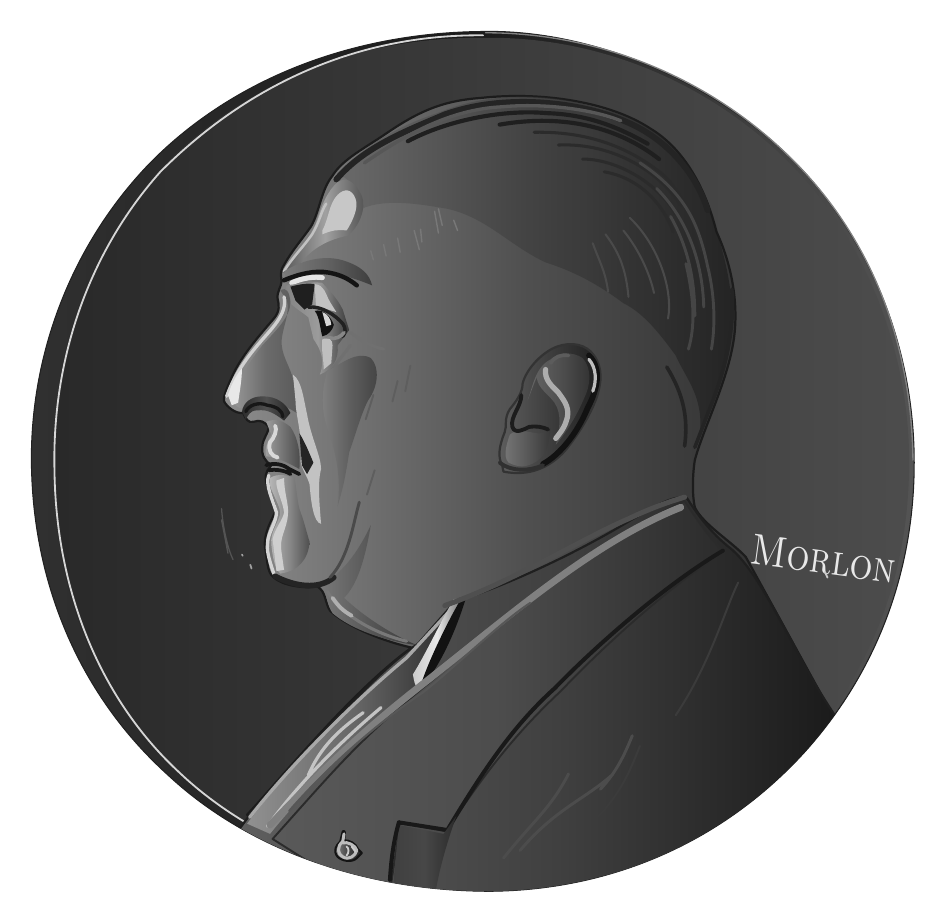
\begin{tikzpicture}[x=0.162mm,y=-0.162mm,line join=round,line cap=round]
  \path[use as bounding box] (79,102) rectangle (778,781);
  % Medal edge and narrow raised lip.
  \path[shade,left color=black!81,right color=black!67,middle color=black!90,draw=black!87,line width=0.38pt] (435,105) .. controls (516,103) and (613,140) .. (680,207)
      .. controls (741,269) and (774,355) .. (774,443) .. controls (774,531) and (743,609) .. (688,670)
      .. controls (625,739) and (539,778) .. (442,779) .. controls (348,779) and (254,749) .. (188,687)
      .. controls (121,626) and (84,541) .. (82,447) .. controls (80,358) and (114,271) .. (175,208)
      .. controls (241,141) and (335,106) .. (435,105) -- cycle;
  \path[shade,left color=black!84,right color=black!70,middle color=black!77] (435,110) .. controls (527,108) and (616,146) .. (679,211)
      .. controls (738,272) and (770,358) .. (770,442) .. controls (770,532) and (740,606) .. (685,669)
      .. controls (622,737) and (533,775) .. (442,775) .. controls (347,775) and (259,743) .. (193,682)
      .. controls (130,624) and (99,538) .. (99,445) .. controls (98,355) and (127,277) .. (183,213)
      .. controls (249,145) and (338,109) .. (435,110) -- cycle;
  \path[draw=black!16,line width=0.66pt] (436,108) .. controls (333,107) and (248,150) .. (183,215)
      .. controls (126,279) and (98,363) .. (100,449) .. controls (101,537) and (132,625) .. (198,686)
      .. controls (257,742) and (350,778) .. (441,777);
  \path[draw=black!49,line width=0.48pt] (438,106) .. controls (531,106) and (616,144) .. (676,203)
      .. controls (742,267) and (772,352) .. (773,441);
  \begin{scope}
  \clip (435,105) .. controls (516,103) and (613,140) .. (680,207)
      .. controls (741,269) and (774,355) .. (774,443) .. controls (774,531) and (743,609) .. (688,670)
      .. controls (625,739) and (539,778) .. (442,779) .. controls (348,779) and (254,749) .. (188,687)
      .. controls (121,626) and (84,541) .. (82,447) .. controls (80,358) and (114,271) .. (175,208)
      .. controls (241,141) and (335,106) .. (435,105) -- cycle;
  % Fine surface marks in the field to the left of the chin.
  \path[draw=black!67,line width=0.46pt] (231,479) .. controls (232,494) and (236,511) .. (240,519) (231,488) -- (236,514);
  \path[draw=black!37,line width=0.62pt] (247,515) -- (247.5,516) (253.5,523) -- (254.5,526);
  % Head and neck in left profile.
  \path[shade,left color=black!45,right color=black!84,middle color=black!69,draw=black!89,line width=0.8pt] (251,719) .. controls (279,689) and (333,622) .. (380,588)
      .. controls (358,583) and (330,572) .. (316,559) .. controls (312,553) and (313,544) .. (306,540)
      .. controls (295,542) and (278,539) .. (272,533) .. controls (266,529) and (267,517) .. (265,509)
      .. controls (264,501) and (268,492) .. (272,484) .. controls (275,479) and (271,473) .. (269,466)
      .. controls (266,460) and (264,454) .. (267,449) -- (270,445)
      .. controls (265,442) and (262,437) .. (263,430) .. controls (263,425) and (268,419) .. (268,415)
      .. controls (265,411) and (261,409) .. (256,411) .. controls (252,412) and (250,409) .. (248,404)
      .. controls (242,405) and (235,399) .. (233,395) .. controls (232,391) and (236,383) .. (239,376)
      .. controls (246,360) and (260,344) .. (272,330) .. controls (277,324) and (276,319) .. (275,315)
      .. controls (274,309) and (278,305) .. (278,301) .. controls (278,297) and (276,294) .. (280,288)
      .. controls (286,277) and (294,268) .. (301,258) .. controls (308,246) and (309,229) .. (318,218)
      .. controls (326,205) and (344,196) .. (360,185) .. controls (389,165) and (408,159) .. (435,157)
      .. controls (482,152) and (535,160) .. (567,181) .. controls (597,199) and (612,234) .. (619,262)
      .. controls (631,288) and (636,317) .. (633,343) .. controls (629,377) and (609,415) .. (602,441)
      .. controls (600,454) and (600,469) .. (602,478) .. controls (608,491) and (631,505) .. (642,517)
      -- (710,641) -- (579,762) -- (348,786) -- cycle;
  % Shoulder, coat, lapels and narrow shirt opening.
  \path[shade,left color=black!63,right color=black!92,middle color=black!75,draw=black!88,line width=0.8pt] (243,733) .. controls (259,710) and (290,674) .. (317,648)
      .. controls (343,621) and (365,598) .. (385,585) -- (414,552)
      .. controls (461,537) and (512,512) .. (552,488) .. controls (568,479) and (586,467) .. (596,471)
      .. controls (603,482) and (614,498) .. (631,511) .. controls (648,526) and (664,558) .. (678,583)
      .. controls (690,607) and (700,623) .. (711,640) -- (748,689) -- (646,787) -- (248,797) -- cycle;
  \path[shade,left color=black!43,right color=black!86,middle color=black!60] (251,726) .. controls (279,689) and (326,636) .. (370,601)
      .. controls (386,588) and (402,571) .. (414,550) -- (421,548)
      .. controls (414,570) and (400,599) .. (386,621) .. controls (350,648) and (302,693) .. (269,734)
      -- cycle;
  \path[draw=black!34,line width=1.2pt] (253,721) .. controls (282,684) and (329,635) .. (376,596) -- (410,559);
  \path[draw=black!23,line width=1.15pt] (267,728) .. controls (289,698) and (318,667) .. (356,635) (299,688)
      .. controls (308,667) and (322,653) .. (342,639);
  \path[shade,left color=black!20,right color=black!54,middle color=black!9] (381,609) .. controls (391,593) and (401,571) .. (413,550) -- (419,549)
      .. controls (408,574) and (398,597) .. (386,621) .. controls (382,618) and (382,614) .. (381,609)
      -- cycle;
  \path[fill=black!93] (387,618) .. controls (392,601) and (408,568) .. (418,551) -- (423,548)
      .. controls (416,570) and (406,597) .. (387,621) -- cycle;
  \path[shade,left color=black!65,right color=black!83,middle color=black!70,draw=black!83,line width=0.7pt] (271,738) .. controls (322,681) and (340,659) .. (392,617)
      .. controls (456,564) and (519,509) .. (594,473) .. controls (601,484) and (614,503) .. (625,513)
      .. controls (589,535) and (538,579) .. (497,622) .. controls (453,663) and (428,701) .. (407,732)
      -- (371,725) -- (364,773) -- (320,769) -- cycle;
  \path[draw=black!50,line width=2.5pt] (269,727) .. controls (313,681) and (343,652) .. (392,614)
      .. controls (458,562) and (523,505) .. (591,478);
  \path[draw=black!66,line width=0.75pt] (284,716) .. controls (312,684) and (349,650) .. (389,623)
      .. controls (412,605) and (451,567) .. (473,553);
  \path[draw=black!90,line width=1.45pt] (370,725) -- (408,731) .. controls (438,681) and (461,648) .. (492,620)
      .. controls (533,578) and (585,535) .. (624,512);
  \path[shade,left color=black!75,right color=black!83,middle color=black!72] (370,727) -- (405,734) -- (415,720) .. controls (407,743) and (402,761) .. (399,778) -- (365,779)
      -- cycle;
  \path[draw=black!91,line width=1.45pt] (363,770) .. controls (364,753) and (366,739) .. (370,725);
  \path[draw=black!70,line width=1.05pt] (452,753) .. controls (477,722) and (489,714) .. (503,687) (465,747)
      .. controls (493,714) and (516,707) .. (538,687) (528,699)
      .. controls (542,684) and (548,669) .. (553,657);
  \path[draw=black!77,line width=0.72pt] (522,725) .. controls (544,703) and (551,685) .. (559,665) (587,641)
      .. controls (614,601) and (626,557) .. (636,537);
  % Hairline, swept hair, the jaw and the ear.
  \path[shade,left color=black!53,right color=black!77,middle color=black!66] (310,539) .. controls (325,529) and (336,517) .. (348,492)
      .. controls (343,521) and (337,539) .. (327,549) .. controls (343,564) and (365,578) .. (384,586)
      .. controls (360,583) and (333,574) .. (318,561) .. controls (314,555) and (314,548) .. (310,539)
      -- cycle;
  \path[draw=black!53,line width=1.1pt] (314,544) .. controls (322,558) and (344,575) .. (376,583);
  \path[draw=black!31,line width=1.4pt] (318,549) .. controls (323,556) and (326,559) .. (333,563);
  \path[draw=black!69,line width=1.8pt] (406,555) .. controls (460,536) and (513,503) .. (550,487)
      .. controls (569,478) and (581,474) .. (594,470);
  \path[opacity=0.54,shade,left color=black!62,right color=black!91,middle color=black!78] (322,216) .. controls (346,191) and (376,177) .. (400,169)
      .. controls (438,153) and (486,152) .. (526,165) .. controls (573,175) and (602,207) .. (614,245)
      .. controls (623,273) and (632,302) .. (631,332) .. controls (632,362) and (617,396) .. (606,422)
      .. controls (609,391) and (596,379) .. (587,359) .. controls (571,337) and (560,325) .. (546,318)
      .. controls (526,303) and (507,293) .. (485,286) .. controls (457,273) and (439,251) .. (408,244)
      .. controls (385,240) and (355,235) .. (337,246) .. controls (341,233) and (336,224) .. (322,216)
      -- cycle;
  \path[draw=black!86,line width=2.15pt] (321,221) .. controls (343,195) and (378,182) .. (406,170)
      .. controls (454,153) and (514,160) .. (551,177) .. controls (580,190) and (603,216) .. (612,245);
  \path[draw=black!66,line width=1.2pt] (343,208) .. controls (375,186) and (410,166) .. (451,164)
      .. controls (484,161) and (522,166) .. (544,175);
  \path[draw=black!88,line width=1.5pt] (377,191) .. controls (409,174) and (453,166) .. (486,169)
      .. controls (518,170) and (542,180) .. (565,193) (449,178)
      .. controls (501,169) and (543,181) .. (574,205);
  \path[draw=black!83,line width=1.1pt] (476,184) .. controls (523,183) and (555,199) .. (578,218)
      .. controls (592,232) and (603,257) .. (607,277) (495,194)
      .. controls (539,192) and (575,216) .. (591,241) (514,205)
      .. controls (541,205) and (573,224) .. (587,248) (531,215)
      .. controls (560,220) and (578,242) .. (585,262);
  \path[draw=black!73,line width=1.05pt] (559,208) .. controls (595,232) and (605,256) .. (612,289)
      .. controls (618,313) and (618,337) .. (615,354) (572,228)
      .. controls (596,252) and (608,285) .. (609,321) (583,250)
      .. controls (597,275) and (602,300) .. (602,328) (595,287)
      .. controls (602,317) and (602,337) .. (597,354);
  \path[draw=black!71,line width=0.74pt] (551,251) .. controls (574,273) and (585,308) .. (581,330) (546,261)
      .. controls (559,277) and (567,296) .. (570,310) (532,264)
      .. controls (544,280) and (548,293) .. (550,313) (522,271)
      .. controls (527,285) and (532,293) .. (534,309);
  \path[draw=black!86,line width=1.3pt] (631,307) .. controls (634,344) and (623,378) .. (612,405) -- (602,431) (580,368)
      .. controls (593,389) and (597,408) .. (594,430);
  \path[shade,left color=black!65,right color=black!69,middle color=black!37] (279,294) .. controls (287,279) and (299,270) .. (305,255)
      .. controls (309,242) and (314,230) .. (322,223) .. controls (330,218) and (336,224) .. (341,234)
      .. controls (345,244) and (338,259) .. (330,265) .. controls (311,269) and (298,277) .. (286,296)
      -- cycle;
  \path[fill=black!22] (310,261) .. controls (315,252) and (315,240) .. (322,233)
      .. controls (327,228) and (333,228) .. (336,236) .. controls (339,243) and (333,255) .. (329,261)
      .. controls (322,260) and (317,261) .. (310,264) -- cycle;
  \path[draw=black!24,line width=0.92pt] (280,293) .. controls (285,284) and (295,274) .. (302,264)
      .. controls (308,254) and (309,246) .. (313,240);
  \path[shade,left color=black!52,right color=black!76,middle color=black!62] (280,293) .. controls (296,283) and (314,280) .. (328,285)
      .. controls (340,289) and (347,295) .. (349,304) .. controls (334,298) and (324,295) .. (315,295)
      .. controls (302,297) and (291,299) .. (282,303) -- cycle;
  \path[draw=black!92,line width=1.6pt] (280,300) .. controls (292,295) and (304,292) .. (315,294)
      .. controls (326,296) and (332,300) .. (337,304);
  \path[draw=black!10,line width=1.8pt] (286,302) .. controls (295,298) and (304,297) .. (310,298);
  \path[draw=black!53,line width=0.52pt] (350,284) -- (348,277);
  \path[draw=black!53,line width=0.52pt] (360,281) -- (358,272);
  \path[draw=black!53,line width=0.52pt] (371,278) -- (369,267);
  \path[draw=black!53,line width=0.52pt] (386,276) -- (382,261);
  \path[draw=black!53,line width=0.52pt] (388,270) -- (387,260);
  \path[draw=black!53,line width=0.52pt] (401,263) -- (398,246);
  \path[draw=black!53,line width=0.52pt] (404,257) -- (401,244);
  \path[draw=black!53,line width=0.52pt] (416,261) -- (413,253);
  \path[shade,left color=black!48,right color=black!78,middle color=black!39] (282,304) .. controls (290,303) and (301,301) .. (310,302)
      .. controls (315,308) and (321,313) .. (326,323) -- (331,339) -- (322,351)
      .. controls (323,362) and (318,370) .. (308,374) .. controls (313,361) and (307,352) .. (303,346)
      -- (299,329) .. controls (293,324) and (285,320) .. (282,314) -- cycle;
  \path[fill=black!88] (285,305) .. controls (293,303) and (299,302) .. (304,303) -- (302,319) -- (296,323) -- (289,316)
      -- cycle;
  \path[fill=black!24] (304,303) .. controls (312,304) and (312,310) .. (316,317) -- (321,325) -- (305,320) -- cycle;
  \path[draw=black!87,line width=1.25pt] (299,321) .. controls (309,320) and (320,327) .. (326,334)
      .. controls (329,339) and (328,341) .. (326,344);
  \path[fill=black!93] (304,324) .. controls (311,322) and (317,329) .. (319,335)
      .. controls (318,339) and (315,343) .. (310,344) .. controls (308,337) and (308,329) .. (304,324)
      -- cycle;
  \path[fill=black!16] (310,325) .. controls (314,326) and (317,331) .. (317,335) -- (313,336) -- cycle;
  \path[draw=black!47,line width=1.3pt] (315,345) .. controls (320,347) and (325,344) .. (327,341);
  \path[fill=black!25] (310,346) .. controls (315,345) and (318,346) .. (318,351) -- (317,365) -- (311,370)
      .. controls (311,361) and (309,355) .. (310,346) -- cycle;
  \path[draw=black!56,line width=1.1pt] (332,341) .. controls (343,349) and (349,352) .. (358,354) (332,351)
      .. controls (324,362) and (319,367) .. (315,375);
  \path[shade,left color=black!49,right color=black!74,middle color=black!63] (314,371) .. controls (326,365) and (337,355) .. (348,361)
      .. controls (355,368) and (354,383) .. (346,394) .. controls (341,403) and (336,421) .. (331,435)
      .. controls (329,448) and (327,461) .. (322,477) .. controls (325,453) and (320,434) .. (315,419)
      .. controls (310,406) and (308,390) .. (314,371) -- cycle;
  \path[draw=black!63,line width=0.7pt] (350,390) -- (344,409) (365,395) -- (369,379) (375,387) -- (379,367) (345,468) -- (351,449);
  \path[shade,left color=black!40,right color=black!65,middle color=black!58] (277,308) .. controls (282,305) and (284,309) .. (285,317)
      .. controls (285,329) and (273,340) .. (263,351) .. controls (251,366) and (245,378) .. (240,390)
      .. controls (239,397) and (244,402) .. (249,400) .. controls (254,394) and (268,390) .. (279,398)
      .. controls (284,401) and (288,402) .. (292,406) .. controls (291,392) and (289,384) .. (286,374)
      .. controls (283,365) and (278,358) .. (278,348) .. controls (279,335) and (285,327) .. (282,315)
      -- cycle;
  \path[draw=black!18,line width=1.18pt] (280,313) .. controls (283,327) and (269,339) .. (260,350)
      .. controls (248,364) and (240,377) .. (235,391);
  \path[fill=black!9] (236,390) .. controls (239,381) and (242,375) .. (247,369)
      .. controls (247,378) and (245,388) .. (244,396) -- (239,398) -- cycle;
  \path[shade,left color=black!82,right color=black!85,middle color=black!69] (247,403) .. controls (248,396) and (254,391) .. (263,391)
      .. controls (274,391) and (281,396) .. (285,404) -- (280,410)
      .. controls (273,405) and (268,401) .. (259,402) .. controls (253,402) and (252,406) .. (250,409)
      -- cycle;
  \path[draw=black!91,line width=1.2pt] (250,403) .. controls (252,398) and (260,395) .. (267,398)
      .. controls (275,399) and (279,403) .. (279,407);
  \path[fill=black!24] (287,374) .. controls (294,379) and (295,392) .. (298,405)
      .. controls (301,423) and (309,438) .. (309,448) .. controls (306,459) and (308,478) .. (309,491)
      .. controls (303,490) and (301,473) .. (300,460) .. controls (298,453) and (294,449) .. (293,442)
      .. controls (295,423) and (289,406) .. (289,395) -- cycle;
  \path[shade,left color=black!36,right color=black!71,middle color=black!54] (266,411) .. controls (273,408) and (279,410) .. (285,415)
      .. controls (291,424) and (293,435) .. (292,448) .. controls (283,443) and (275,439) .. (266,438)
      .. controls (264,432) and (268,425) .. (270,421) -- cycle;
  \path[draw=black!15,line width=1.4pt] (273,414) .. controls (275,417) and (272,424) .. (269,427)
      .. controls (267,433) and (270,438) .. (275,439);
  \path[fill=black!86] (292,420) .. controls (296,426) and (300,436) .. (303,443) -- (298,452) -- (294,445) -- cycle;
  \path[draw=black!91,line width=1.35pt] (266,445) .. controls (272,443) and (279,444) .. (284,448) -- (292,452) (268,449)
      .. controls (273,448) and (281,449) .. (285,452);
  \path[shade,left color=black!29,right color=black!69,middle color=black!47] (269,455) .. controls (275,451) and (283,453) .. (288,455)
      .. controls (290,462) and (290,475) .. (293,482) .. controls (296,490) and (298,499) .. (300,505)
      .. controls (299,519) and (291,528) .. (277,530) .. controls (272,525) and (271,516) .. (270,507)
      .. controls (269,498) and (275,491) .. (277,483) .. controls (277,477) and (271,468) .. (269,461)
      -- cycle;
  \path[draw=black!17,line width=1.2pt] (268,453) .. controls (265,460) and (271,472) .. (274,482)
      .. controls (274,490) and (267,498) .. (267,507) .. controls (266,513) and (270,524) .. (272,530);
  \path[fill=black!19] (271,503) .. controls (273,494) and (279,488) .. (280,482)
      .. controls (279,473) and (273,463) .. (274,457) -- (280,455)
      .. controls (280,467) and (284,476) .. (283,484) .. controls (282,496) and (276,501) .. (278,513)
      -- (280,527) -- (274,528) -- cycle;
  \path[draw=black!86,line width=2pt] (273,532) .. controls (288,540) and (307,543) .. (319,533);
  \path[draw=black!71,line width=1.05pt] (316,533) .. controls (331,517) and (334,491) .. (339,474);
  \path[shade,left color=black!63,right color=black!89,middle color=black!76,draw=black!80,line width=0.8pt] (451,445) .. controls (447,438) and (449,429) .. (453,419)
      .. controls (455,414) and (452,409) .. (457,401) .. controls (462,395) and (467,388) .. (467,381)
      .. controls (470,369) and (483,356) .. (494,352) .. controls (505,348) and (517,350) .. (523,359)
      .. controls (530,369) and (529,380) .. (525,392) .. controls (520,406) and (510,422) .. (500,434)
      .. controls (488,447) and (472,454) .. (452,450) -- cycle;
  \path[shade,left color=black!53,right color=black!78,middle color=black!65] (456,443) .. controls (451,438) and (455,427) .. (457,421)
      .. controls (462,417) and (467,418) .. (473,419) .. controls (481,421) and (485,420) .. (489,416)
      .. controls (487,428) and (487,436) .. (478,442) .. controls (470,447) and (464,447) .. (456,443)
      -- cycle;
  \path[shade,left color=black!60,right color=black!81,middle color=black!69] (471,394) .. controls (475,383) and (477,368) .. (489,362)
      .. controls (495,356) and (507,356) .. (514,361) .. controls (522,370) and (520,383) .. (515,393)
      .. controls (509,407) and (502,418) .. (493,429) .. controls (496,417) and (498,405) .. (492,396)
      .. controls (487,389) and (479,385) .. (478,376) -- cycle;
  \path[draw=black!93,line width=2.05pt] (519,359) .. controls (530,370) and (525,387) .. (518,400)
      .. controls (510,420) and (496,437) .. (483,444);
  \path[draw=black!25,line width=1.15pt] (519,362) .. controls (525,369) and (525,379) .. (522,387);
  \path[draw=black!32,line width=1.9pt] (485,370) .. controls (484,378) and (490,383) .. (495,388)
      .. controls (500,395) and (505,401) .. (501,411) .. controls (499,417) and (496,420) .. (493,424);
  \path[draw=black!89,line width=1.4pt] (466,390) .. controls (466,399) and (457,407) .. (459,415)
      .. controls (461,421) and (468,417) .. (472,415) .. controls (477,414) and (483,415) .. (487,417);
  \path[draw=black!81,line width=1.4pt] (449,443) .. controls (458,450) and (472,450) .. (483,445);
  \path[draw=black!64,line width=1.3pt] (489,365) .. controls (492,360) and (497,358) .. (503,359);
  % Signature in relief. The initial is larger than the five following capitals.
  \node[anchor=base west,inner sep=0pt,outer sep=0pt,text=black!9,rotate=-7.8] at (645,522) {\resizebox{18.5mm}{3.79mm}{\textsc{Morlon}}};
  \path[draw=black!21,line width=0.68pt] (704.1,528.8) -- (706,533.1);
  % Small looped device on the coat at the lower rim.
  \path[shade,left color=black!44,right color=black!85,middle color=black!72,draw=black!92,line width=0.75pt] (324,740) -- (326,732) .. controls (328,731) and (328,733) .. (327,739)
      .. controls (331,739) and (336,741) .. (338,746) -- (341,749) -- (337,753)
      .. controls (333,757) and (325,755) .. (322,752) .. controls (318,747) and (321,743) .. (324,740)
      -- cycle;
  \path[draw=black!26,line width=1.08pt] (327,734) -- (326,740) .. controls (321,744) and (322,750) .. (326,752)
      .. controls (331,755) and (336,751) .. (337,747) .. controls (336,743) and (330,740) .. (326,741);
  \path[draw=black!20,line width=0.67pt] (329,744) .. controls (331,745) and (331,749) .. (329,751) (333,744) -- (336,748);
  \end{scope}
\end{tikzpicture}%
}
\clearpage
\scanpage{3}
% crop-candidate: scan 3
\figure{%
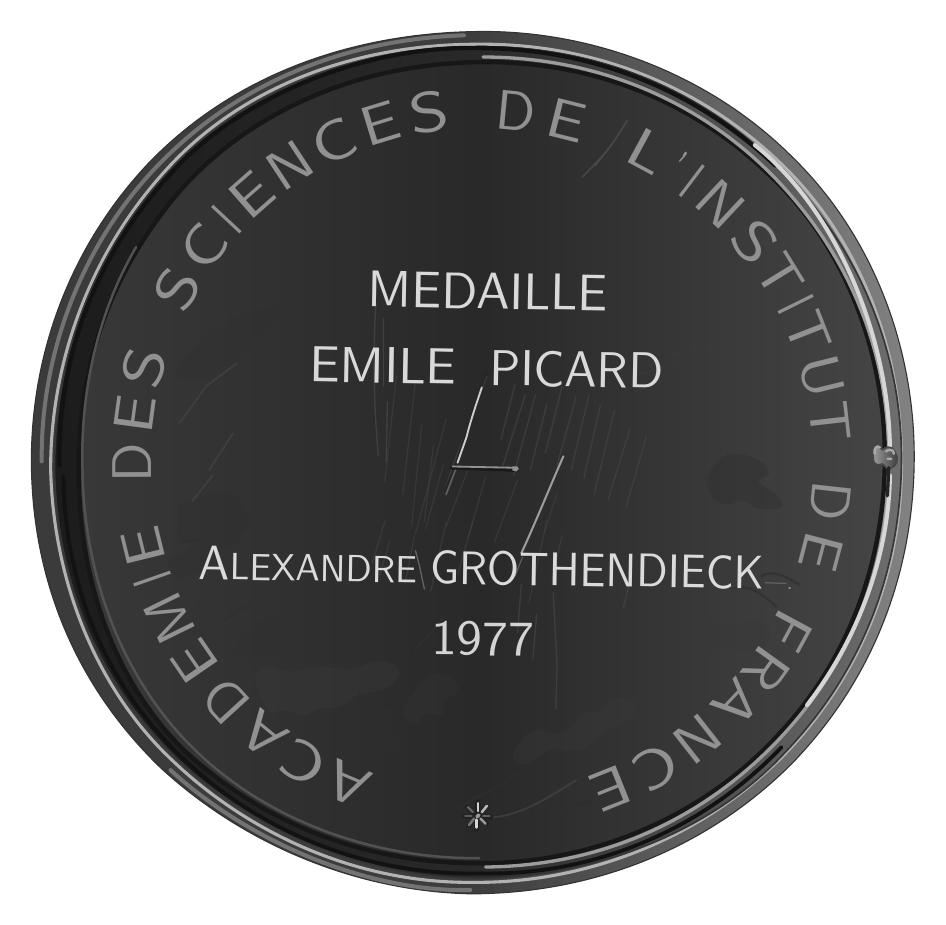
\begin{tikzpicture}[x=0.162mm,y=-0.162mm,line join=round,line cap=round]
  \path[use as bounding box] (65,114) rectangle (763,795);
  % Outer edge, concentric mouldings and inner field.
  \path[shade,left color=black!77,right color=black!49,middle color=black!76,draw=black!80,line width=0.4pt] (419,117) .. controls (508,116) and (600,151) .. (664,215)
      .. controls (728,277) and (760,365) .. (760,450) .. controls (760,542) and (727,626) .. (664,691)
      .. controls (596,759) and (506,793) .. (412,793) .. controls (322,791) and (234,754) .. (169,694)
      .. controls (105,632) and (70,552) .. (68,461) .. controls (66,372) and (98,286) .. (159,221)
      .. controls (226,151) and (319,118) .. (419,117) -- cycle;
  \path[draw=black!55,line width=1.45pt] (76,454) .. controls (75,362) and (113,275) .. (172,217)
      .. controls (233,156) and (316,123) .. (407,120) (412,790)
      .. controls (333,792) and (239,753) .. (177,696);
  \path[draw=black!30,line width=1.12pt] (83,460) .. controls (83,373) and (116,288) .. (174,225)
      .. controls (231,162) and (318,128) .. (413,127) .. controls (508,125) and (593,160) .. (656,221)
      .. controls (717,280) and (750,365) .. (750,453) .. controls (751,538) and (720,620) .. (658,684)
      .. controls (595,748) and (505,785) .. (414,784) .. controls (325,785) and (240,747) .. (179,689)
      .. controls (119,633) and (85,548) .. (83,460);
  \path[shade,left color=black!89,right color=black!57,middle color=black!84,draw=black!79,line width=0.6pt] (418,129) .. controls (507,128) and (591,160) .. (653,223)
      .. controls (716,284) and (750,367) .. (750,451) .. controls (750,541) and (718,621) .. (657,684)
      .. controls (598,747) and (504,781) .. (416,781) .. controls (329,780) and (244,744) .. (184,689)
      .. controls (118,626) and (87,544) .. (86,457) .. controls (87,368) and (118,288) .. (177,225)
      .. controls (238,160) and (328,130) .. (418,129) -- cycle;
  \path[draw=black!93,line width=1.55pt] (90,457) .. controls (88,363) and (125,282) .. (184,221)
      .. controls (236,168) and (328,128) .. (418,130) .. controls (508,130) and (589,163) .. (651,222);
  \path[draw=black!93,line width=1.38pt] (93,466) .. controls (94,555) and (129,634) .. (190,690)
      .. controls (249,745) and (332,779) .. (420,777) .. controls (507,779) and (593,744) .. (656,678);
  \path[shade,left color=black!78,right color=black!73,middle color=black!84,draw=black!91,line width=1.6pt] (420,141) .. controls (504,140) and (584,169) .. (647,230)
      .. controls (707,286) and (737,370) .. (737,451) .. controls (737,533) and (708,613) .. (649,673)
      .. controls (589,736) and (502,770) .. (418,769) .. controls (330,769) and (251,739) .. (187,680)
      .. controls (132,625) and (104,545) .. (105,456) .. controls (105,376) and (132,302) .. (186,240)
      .. controls (243,177) and (328,142) .. (420,141) -- cycle;
  \path[draw=black!39,line width=1.2pt] (422,137) .. controls (511,137) and (591,171) .. (649,230)
      .. controls (705,287) and (739,361) .. (740,447) .. controls (741,539) and (711,612) .. (652,674)
      .. controls (591,737) and (513,771) .. (424,772);
  \path[draw=black!16,line width=1.45pt] (635,206) .. controls (699,257) and (740,356) .. (741,444) (741,465)
      .. controls (740,529) and (716,593) .. (676,645);
  \path[draw=black!68,line width=0.9pt] (150,286) .. controls (120,337) and (106,400) .. (108,461)
      .. controls (109,542) and (138,621) .. (191,675) .. controls (249,735) and (336,766) .. (419,765);
  \begin{scope}
  \clip (420,141) .. controls (504,140) and (584,169) .. (647,230)
      .. controls (707,286) and (737,370) .. (737,451) .. controls (737,533) and (708,613) .. (649,673)
      .. controls (589,736) and (502,770) .. (418,769) .. controls (330,769) and (251,739) .. (187,680)
      .. controls (132,625) and (104,545) .. (105,456) .. controls (105,376) and (132,302) .. (186,240)
      .. controls (243,177) and (328,142) .. (420,141) -- cycle;
  % Worn areas of the field and the principal visible scores.
  \path[opacity=0.3,fill=black!81] (185,375) .. controls (213,347) and (230,334) .. (266,332)
      .. controls (248,349) and (239,369) .. (224,376) .. controls (213,381) and (202,393) .. (191,392)
      -- (181,386) -- cycle;
  \path[opacity=0.3,fill=black!82] (183,488) .. controls (205,480) and (219,475) .. (229,481) -- (241,501) -- (229,518) -- (210,527)
      -- (203,540) -- (182,546) -- (174,534) -- (194,519) -- (182,515) -- cycle;
  \path[opacity=0.3,fill=black!80] (201,552) .. controls (227,540) and (240,543) .. (250,536) -- (273,539) -- (270,553) -- (255,564)
      -- (237,573) -- (223,577) -- (207,592) -- (192,587) -- cycle;
  \path[opacity=0.3,fill=black!81] (235,586) .. controls (264,569) and (289,562) .. (319,566) -- (331,578) -- (303,591) -- (285,592)
      -- (265,606) -- (251,604) -- (238,612) -- (227,602) -- cycle;
  \path[opacity=0.3,fill=black!76] (245.85,633.75) .. controls (241.95,623.25) and (242.85,617.40) .. (250.45,615.80)
      .. controls (256.15,614.60) and (260.95,614.90) .. (266.15,617.30)
      .. controls (270.05,619.10) and (275.30,619.10) .. (284.10,616.70)
      .. controls (290.70,614.90) and (297.75,614.60) .. (307.75,616.20)
      .. controls (315.25,617.40) and (322.30,616.50) .. (331.10,612.50)
      .. controls (337.70,609.50) and (343.85,609.35) .. (351.45,612.95)
      .. controls (357.15,615.65) and (358.05,619.55) .. (352.85,626.35)
      .. controls (348.95,631.45) and (343.25,634.30) .. (333.25,635.10)
      .. controls (325.75,635.70) and (320.20,637.80) .. (315.40,642.60)
      .. controls (311.80,646.20) and (307.00,647.85) .. (299.00,647.45)
      .. controls (293.00,647.15) and (289.10,648.20) .. (286.70,651.40)
      .. controls (284.90,653.80) and (281.30,653.95) .. (274.10,651.15)
      .. controls (268.70,649.05) and (264.05,648.75) .. (258.85,650.75)
      .. controls (254.95,652.25) and (251.05,647.75) .. (245.85,633.75) -- cycle;
  \path[opacity=0.3,fill=black!81] (289.80,668.05) .. controls (282.60,665.35) and (283.20,660.85) .. (294.40,652.45)
      .. controls (302.80,646.15) and (309.85,644.35) .. (317.45,647.95)
      .. controls (323.15,650.65) and (328.40,650.65) .. (334.80,647.05)
      .. controls (339.60,644.35) and (343.95,644.50) .. (349.15,648.50)
      .. controls (353.05,651.50) and (354.25,654.80) .. (352.25,659.60)
      .. controls (350.75,663.20) and (352.25,666.50) .. (358.25,670.50)
      .. controls (362.75,673.50) and (363.20,676.65) .. (358.40,681.05)
      .. controls (354.80,684.35) and (349.25,684.35) .. (339.25,679.95)
      .. controls (331.75,676.65) and (325.75,676.50) .. (319.75,680.50)
      .. controls (315.25,683.50) and (311.50,683.20) .. (307.50,678.40)
      .. controls (304.50,674.80) and (299.40,671.65) .. (289.80,668.05) -- cycle;
  \path[opacity=0.3,fill=black!79] (361.75,656.40) .. controls (357.25,652.80) and (358.75,646.05) .. (368.75,632.85)
      .. controls (376.25,622.95) and (383.00,618.90) .. (391.00,621.30)
      .. controls (397.00,623.10) and (400.60,625.65) .. (402.20,630.05)
      .. controls (403.40,633.35) and (401.90,636.05) .. (396.30,638.85)
      .. controls (392.10,640.95) and (390.30,643.80) .. (391.10,648.60)
      .. controls (391.70,652.20) and (389.45,653.55) .. (382.65,652.35)
      .. controls (377.55,651.45) and (374.25,652.80) .. (372.25,657.60)
      .. controls (370.75,661.20) and (367.75,661.20) .. (361.75,656.40) -- cycle;
  \path[opacity=0.3,fill=black!77] (447.85,689.50) .. controls (443.95,686.50) and (444.85,681.55) .. (452.45,672.35)
      .. controls (458.15,665.45) and (464.75,663.20) .. (474.75,666.40)
      .. controls (482.25,668.80) and (488.25,666.85) .. (494.25,658.45)
      .. controls (498.75,652.15) and (503.10,649.30) .. (508.70,650.10)
      .. controls (512.90,650.70) and (516.35,648.90) .. (519.95,643.30)
      .. controls (522.65,639.10) and (527.00,637.90) .. (535.00,640.30)
      .. controls (541.00,642.10) and (543.10,645.10) .. (540.70,650.70)
      .. controls (538.90,654.90) and (534.55,658.50) .. (525.35,662.50)
      .. controls (518.45,665.50) and (512.45,669.40) .. (505.65,675.80)
      .. controls (500.55,680.60) and (494.40,682.10) .. (484.80,679.70)
      .. controls (477.60,677.90) and (471.15,679.70) .. (463.55,686.90)
      .. controls (457.85,692.30) and (453.05,693.50) .. (447.85,689.50) -- cycle;
  \path[opacity=0.3,fill=black!78] (566.20,601.70) .. controls (561.40,599.90) and (562.15,596.45) .. (570.55,589.65)
      .. controls (576.85,584.55) and (583.30,581.70) .. (592.10,580.90)
      .. controls (598.70,580.30) and (603.50,580.60) .. (607.50,582.20)
      .. controls (610.50,583.40) and (615.00,582.95) .. (623.00,580.15)
      .. controls (629.00,578.05) and (634.55,577.90) .. (641.35,580.30)
      .. controls (646.45,582.10) and (648.55,585.40) .. (647.35,591.80)
      .. controls (646.45,596.60) and (643.00,599.75) .. (635.00,601.75)
      .. controls (629.00,603.25) and (623.00,602.95) .. (615.00,600.15)
      .. controls (609.00,598.05) and (603.45,598.65) .. (596.65,603.05)
      .. controls (591.55,606.35) and (586.90,607.55) .. (581.30,606.35)
      .. controls (577.10,605.45) and (572.60,604.10) .. (566.20,601.70) -- cycle;
  \path[opacity=0.3,fill=black!83] (598.75,466.00) .. controls (600.25,460.00) and (603.25,455.35) .. (609.25,450.95)
      .. controls (613.75,447.65) and (619.45,446.90) .. (628.65,449.30)
      .. controls (635.55,451.10) and (640.50,453.95) .. (644.50,459.15)
      .. controls (647.50,463.05) and (646.75,465.60) .. (640.75,467.20)
      .. controls (636.25,468.40) and (636.70,470.50) .. (643.90,474.50)
      .. controls (649.30,477.50) and (653.20,480.80) .. (656.40,485.60)
      .. controls (658.80,489.20) and (656.40,491.15) .. (646.80,491.55)
      .. controls (639.60,491.85) and (634.50,490.65) .. (630.50,487.05)
      .. controls (627.50,484.35) and (623.75,484.05) .. (617.75,486.85)
      .. controls (613.25,488.95) and (608.75,488.05) .. (602.75,482.85)
      .. controls (598.25,478.95) and (596.75,474.00) .. (598.75,466.00) -- cycle;
  \path[opacity=0.67,draw=black!71,line width=0.48pt] (338,331) .. controls (335,375) and (337,419) .. (340,450) (344,342) -- (344,395) (347,407)
      -- (346,454);
  \path[opacity=0.67,draw=black!76,line width=0.48pt] (354,387) -- (345,470) (369,391) -- (359,480) (374,425) -- (366,504) (383,442) -- (376,501);
  \path[opacity=0.67,draw=black!73,line width=0.47pt] (425,387) -- (400,453) -- (391,479) (447,394) -- (436,437) (455,402) -- (436,462) (463,402)
      -- (446,465) (472,409) -- (459,461);
  \path[opacity=0.67,draw=black!73,line width=0.45pt] (484,395) -- (471,447) (495,403) -- (480,457) (505,402) -- (491,461) (514,410) -- (501,467)
      (525,414) -- (509,480) (537,429) -- (520,484) (550,435) -- (534,490);
  \path[opacity=0.67,draw=black!75,line width=0.4pt] (393,421) -- (369,511) (391,456) -- (377,507) (410,461) -- (393,505) (424,466) -- (410,515)
      (449,469) -- (431,517) (480,479) -- (470,510);
  \path[opacity=0.67,draw=black!75,line width=0.45pt] (345,501) -- (335,534) (349,516) -- (341,543) (368,513) -- (361,550) (393,502) -- (381,556)
      (414,501) -- (402,543) (472,500) -- (458,565) (484,512) -- (476,547);
  \path[opacity=0.67,draw=black!73,line width=0.5pt] (477,557) -- (480,614) -- (479,648) (452,550) -- (449,588) (464,574) -- (461,609) (537,548)
      -- (532,569);
  \path[opacity=0.67,draw=black!77,line width=0.47pt] (551,379) -- (575,369) -- (604,365) (544,386) -- (582,374) (541,399) -- (575,386);
  \path[opacity=0.67,draw=black!73,line width=0.65pt] (184,424) -- (205,395) -- (229,377) (207,461) -- (226,432) (194,485) -- (210,465) (430,733)
      .. controls (455,731) and (478,714) .. (495,704);
  \path[opacity=0.67,draw=black!68,line width=0.61pt] (535,187) -- (524,204) -- (510,222) (519,211) -- (500,231);
  \path[opacity=0.67,draw=black!82,line width=0.86pt] (402,726) .. controls (418,716) and (451,701) .. (463,688) (452,748) -- (481,731) -- (507,719);
  \path[opacity=0.67,draw=black!81,line width=0.87pt] (184,518) -- (201,514) -- (211,509) (219,578) -- (240,566) (369,602) -- (390,577) (617,554)
      .. controls (629,549) and (641,558) .. (652,568) (640,544)
      .. controls (648,539) and (658,543) .. (670,551);
  \path[draw=black!85,line width=0.95pt] (425,384) .. controls (420,393) and (416,411) .. (410,427) -- (401,456) -- (392,478);
  \path[draw=black!20,line width=0.69pt] (421,396) .. controls (416,411) and (412,423) .. (409,435) -- (402,455);
  \path[draw=black!62,line width=0.6pt] (401,459) -- (393,480);
  \path[draw=black!82,line width=1.15pt] (487,449) .. controls (479,468) and (463,504) .. (452,530) -- (445,547);
  \path[draw=black!38,line width=0.73pt] (485,450) .. controls (479,463) and (464,500) .. (452,526);
  \path[draw=black!64,line width=0.43pt] (453,529) -- (447,544);
  \path[draw=black!61,line width=0.48pt] (369,524) .. controls (371,531) and (373,539) .. (374,545) -- (376,554);
  % Short rule between the award title and the recipient.
  \path[draw=black!90,line width=1.18pt] (397,459) -- (449,461);
  \path[draw=black!43,line width=0.66pt] (398,458) -- (447,459);
  \path[fill=black!44] (445,458) -- (449,458) -- (450,460) -- (448,462) -- (445,461) -- cycle;
  % Circular legend, clockwise: ACADEMIE DES SCIENCES DE L'INSTITUT DE FRANCE
  % ACADEMIE
  \node[anchor=base,inner sep=0pt,outer sep=0pt,text=black!43,rotate=157] at (321.86,692.98) {\resizebox{5.508mm}{4.93mm}{\sffamily A}};
  \node[anchor=base,inner sep=0pt,outer sep=0pt,text=black!43,rotate=149] at (289.65,677.45) {\resizebox{5.508mm}{4.93mm}{\sffamily C}};
  \node[anchor=base,inner sep=0pt,outer sep=0pt,text=black!43,rotate=140.8] at (259.19,656.69) {\resizebox{5.508mm}{4.93mm}{\sffamily A}};
  \node[anchor=base,inner sep=0pt,outer sep=0pt,text=black!43,rotate=132.5] at (231.65,631.25) {\resizebox{5.022mm}{4.93mm}{\sffamily D}};
  \node[anchor=base,inner sep=0pt,outer sep=0pt,text=black!43,rotate=124.4] at (208.62,602.59) {\resizebox{4.86mm}{4.93mm}{\sffamily E}};
  \node[anchor=base,inner sep=0pt,outer sep=0pt,text=black!43,rotate=116.2] at (189.65,570.41) {\resizebox{6.156mm}{4.93mm}{\sffamily M}};
  \node[anchor=base,inner sep=0pt,outer sep=0pt,text=black!43,rotate=109.2] at (177.28,540.91) {\resizebox{1.296mm}{4.93mm}{\sffamily I}};
  \node[anchor=base,inner sep=0pt,outer sep=0pt,text=black!43,rotate=103.8] at (169.98,517.27) {\resizebox{4.86mm}{4.93mm}{\sffamily E}};
  % DES
  \node[anchor=base,inner sep=0pt,outer sep=0pt,text=black!43,rotate=90.2] at (162.1,455.42) {\resizebox{5.022mm}{4.93mm}{\sffamily D}};
  \node[anchor=base,inner sep=0pt,outer sep=0pt,text=black!43,rotate=82.3] at (163.84,419.11) {\resizebox{4.86mm}{4.93mm}{\sffamily E}};
  \node[anchor=base,inner sep=0pt,outer sep=0pt,text=black!43,rotate=74.6] at (170.84,384.35) {\resizebox{5.022mm}{4.93mm}{\sffamily S}};
  % SCIENCES
  \node[anchor=base,inner sep=0pt,outer sep=0pt,text=black!43,rotate=60.8] at (195.41,326.12) {\resizebox{5.022mm}{4.93mm}{\sffamily S}};
  \node[anchor=base,inner sep=0pt,outer sep=0pt,text=black!43,rotate=52.7] at (215.47,295.04) {\resizebox{5.346mm}{4.93mm}{\sffamily C}};
  \node[anchor=base,inner sep=0pt,outer sep=0pt,text=black!43,rotate=47] at (232.01,274.97) {\resizebox{1.296mm}{4.93mm}{\sffamily I}};
  \node[anchor=base,inner sep=0pt,outer sep=0pt,text=black!43,rotate=41.3] at (250.56,256.81) {\resizebox{5.022mm}{4.93mm}{\sffamily E}};
  \node[anchor=base,inner sep=0pt,outer sep=0pt,text=black!43,rotate=33.4] at (279.04,234.98) {\resizebox{5.508mm}{4.93mm}{\sffamily N}};
  \node[anchor=base,inner sep=0pt,outer sep=0pt,text=black!43,rotate=25.2] at (311.39,216.77) {\resizebox{5.508mm}{4.93mm}{\sffamily C}};
  \node[anchor=base,inner sep=0pt,outer sep=0pt,text=black!43,rotate=17] at (346.01,203.63) {\resizebox{4.86mm}{4.93mm}{\sffamily E}};
  \node[anchor=base,inner sep=0pt,outer sep=0pt,text=black!43,rotate=8.9] at (381.62,195.73) {\resizebox{5.022mm}{4.93mm}{\sffamily S}};
  % DE
  \node[anchor=base,inner sep=0pt,outer sep=0pt,text=black!43,rotate=-5.5] at (446.14,194.49) {\resizebox{5.022mm}{4.93mm}{\sffamily D}};
  \node[anchor=base,inner sep=0pt,outer sep=0pt,text=black!43,rotate=-14.1] at (484.16,201.06) {\resizebox{4.86mm}{4.93mm}{\sffamily E}};
  % L'INSTITUT
  \node[anchor=base,inner sep=0pt,outer sep=0pt,text=black!43,rotate=-28.4] at (543.97,224.37) {\resizebox{4.698mm}{4.93mm}{\sffamily L}};
  \node[anchor=base,inner sep=0pt,outer sep=0pt,text=black!43,rotate=-33.8] at (564.75,237.1) {\resizebox{1.134mm}{4.93mm}{\sffamily \textquoteright}};
  \node[anchor=base,inner sep=0pt,outer sep=0pt,text=black!43,rotate=-37.2] at (577.18,246.11) {\resizebox{1.296mm}{4.93mm}{\sffamily I}};
  \node[anchor=base,inner sep=0pt,outer sep=0pt,text=black!43,rotate=-43.2] at (598.04,263.49) {\resizebox{5.508mm}{4.93mm}{\sffamily N}};
  \node[anchor=base,inner sep=0pt,outer sep=0pt,text=black!43,rotate=-51.5] at (623.65,291.13) {\resizebox{5.022mm}{4.93mm}{\sffamily S}};
  \node[anchor=base,inner sep=0pt,outer sep=0pt,text=black!43,rotate=-58.4] at (641.84,316.78) {\resizebox{5.184mm}{4.93mm}{\sffamily T}};
  \node[anchor=base,inner sep=0pt,outer sep=0pt,text=black!43,rotate=-63.7] at (653.69,337.91) {\resizebox{1.296mm}{4.93mm}{\sffamily I}};
  \node[anchor=base,inner sep=0pt,outer sep=0pt,text=black!43,rotate=-68.6] at (662.64,358.48) {\resizebox{5.184mm}{4.93mm}{\sffamily T}};
  \node[anchor=base,inner sep=0pt,outer sep=0pt,text=black!43,rotate=-76.1] at (672.92,391.29) {\resizebox{5.346mm}{4.93mm}{\sffamily U}};
  \node[anchor=base,inner sep=0pt,outer sep=0pt,text=black!43,rotate=-83.5] at (679.13,424.68) {\resizebox{5.184mm}{4.93mm}{\sffamily T}};
  % DE
  \node[anchor=base,inner sep=0pt,outer sep=0pt,text=black!43,rotate=-96.3] at (679.33,483.42) {\resizebox{5.022mm}{4.93mm}{\sffamily D}};
  \node[anchor=base,inner sep=0pt,outer sep=0pt,text=black!43,rotate=-104.7] at (672.31,521.35) {\resizebox{4.86mm}{4.93mm}{\sffamily E}};
  % FRANCE
  \node[anchor=base,inner sep=0pt,outer sep=0pt,text=black!43,rotate=-118.4] at (649.33,579.66) {\resizebox{4.698mm}{4.93mm}{\sffamily F}};
  \node[anchor=base,inner sep=0pt,outer sep=0pt,text=black!43,rotate=-125.7] at (631.5,607.82) {\resizebox{5.184mm}{4.93mm}{\sffamily R}};
  \node[anchor=base,inner sep=0pt,outer sep=0pt,text=black!43,rotate=-133.1] at (609.88,633.61) {\resizebox{5.508mm}{4.93mm}{\sffamily A}};
  \node[anchor=base,inner sep=0pt,outer sep=0pt,text=black!43,rotate=-141.8] at (580.74,660.1) {\resizebox{5.508mm}{4.93mm}{\sffamily N}};
  \node[anchor=base,inner sep=0pt,outer sep=0pt,text=black!43,rotate=-150] at (550,680.63) {\resizebox{5.508mm}{4.93mm}{\sffamily C}};
  \node[anchor=base,inner sep=0pt,outer sep=0pt,text=black!43,rotate=-158.2] at (516.68,696.28) {\resizebox{4.86mm}{4.93mm}{\sffamily E}};
  % Central inscriptions, top to bottom.
  \node[anchor=base west,inner sep=0pt,outer sep=0pt,text=black!15,rotate=-1] at (331.6,332.8) {\resizebox{30.45mm}{4.53mm}{\sffamily MEDAILLE}};
  \node[anchor=base west,inner sep=0pt,outer sep=0pt,text=black!15,rotate=-1] at (285.6,391.4) {\resizebox{18.7mm}{4.46mm}{\sffamily EMILE}};
  \node[anchor=base west,inner sep=0pt,outer sep=0pt,text=black!15,rotate=-1] at (426.8,394.3) {\resizebox{22.1mm}{4.45mm}{\sffamily PICARD}};
  % ALEXANDRE GROTHENDIECK
  % Smaller capitals after the initial A.
  \node[anchor=base west,inner sep=0pt,outer sep=0pt,text=black!14,rotate=-0.94] at (199,546.5) {\resizebox{27.7mm}{4.27mm}{\sffamily A\scalebox{0.78}{LEXANDRE}}};
  \node[anchor=base west,inner sep=0pt,outer sep=0pt,text=black!14,rotate=-0.94] at (380.3,549.8) {\resizebox{42.4mm}{4.15mm}{\sffamily GROTHENDIECK}};
  % Beside the foot of K: empty first alternative for a surface fleck, then a possible stop.
  \node[anchor=base west,inner sep=0pt,outer sep=0pt,text=black!40,rotate=-0.94] at (642.7,554) {\scriptsize\unsure{{}|.}};
  \node[anchor=base west,inner sep=0pt,outer sep=0pt,text=black!17,rotate=-0.4] at (381.2,605.6) {\resizebox{13.1mm}{4.1mm}{\sffamily 1977}};
  % Small radial ornament in the gap between the ends of the circular legend.
  \path[fill=black!87] (414,730) .. controls (413,726) and (411,724) .. (408,723)
      .. controls (407,726) and (410,729) .. (414,731) -- (405,731)
      .. controls (405,735) and (411,735) .. (414,733) .. controls (411,737) and (409,739) .. (409,741)
      .. controls (413,742) and (416,737) .. (416,734) .. controls (416,738) and (414,741) .. (415,744)
      .. controls (420,745) and (420,739) .. (419,734) .. controls (422,737) and (423,740) .. (426,740)
      .. controls (428,737) and (425,735) .. (421,733) .. controls (424,734) and (428,736) .. (430,733)
      .. controls (430,730) and (425,730) .. (421,731) .. controls (425,728) and (427,725) .. (426,722)
      .. controls (422,722) and (421,726) .. (419,730) .. controls (420,727) and (421,722) .. (419,719)
      .. controls (415,718) and (415,723) .. (416,730) -- cycle;
  \path[draw=black!18,line width=1.05pt] (418,722) -- (418,728);
  \path[draw=black!29,line width=0.95pt] (425,724) -- (421,729);
  \path[draw=black!61,line width=0.87pt] (427,732) -- (422,732);
  \path[draw=black!40,line width=0.88pt] (424,738) -- (420,734);
  \path[draw=black!17,line width=1.05pt] (417,741) -- (417,735);
  \path[draw=black!55,line width=0.94pt] (411,739) -- (415,734);
  \path[draw=black!65,line width=0.85pt] (408,732) -- (413,732);
  \path[draw=black!61,line width=0.82pt] (410,725) -- (414,729);
  \path[fill=black!39] (416,732) -- (418,730) -- (420,731) -- (419,733) -- (417,734) -- cycle;
  \end{scope}
  % Small interruption in the rim at the right.
  \path[shade,left color=black!38,right color=black!77,middle color=black!58,draw=black!72,line width=0.6pt] (728,449) .. controls (727,444) and (729,440) .. (732,441) -- (735,445)
      .. controls (741,440) and (744,444) .. (746,449) .. controls (748,452) and (746,458) .. (742,459)
      .. controls (739,462) and (737,457) .. (735,456) .. controls (732,458) and (728,456) .. (728,453)
      -- cycle;
  \path[draw=black!34,line width=0.9pt] (729,448) .. controls (728,444) and (731,441) .. (733,443) (738,446)
      .. controls (741,444) and (744,445) .. (744,448) (739,452) -- (742,452);
  \path[draw=black!86,line width=1.2pt] (740,459) -- (739,481);
\end{tikzpicture}%
}
